\subsection{Front Door}

Nachdem der \nameref{sec:integration-reverse-proxy} den Zugriff auf verteilte (HTTP-)Ressourcen vereinfacht hat, soll nun das \emph{Front Door} Pattern einen gesamtheitlichen Authentication-Mechanismus sowie Session-Kontext über alles Systemkomponenten ermöglichen.

\subsection*{Kontext}
In einem System bestehend aus mehreren Webapplikationen soll ein \nameref{sec:integration-reverse-proxy} die Authentication aller Benutzer generalisiert übernehmen.

\subsection*{Problem}
Die verschiedenen Komponenten im System verwalten im Normalfall jeweils eigene Datenbanken mit Benutzerinformationen. Wie kann für ein solches System ein Single Sign On umgesetzt werden, wobei auf folgende Faktoren zu achten ist:

\begin{itemize}
	\item Bestehende Komponenten sollen weiterhin auch ihre eigenen Datenbanken verwenden können
	\item Es soll nicht für jede Komponente erneut nach einem Passwort o.Ä. gefragt werden (wobei dies je nach Sicherheitsrichtlinie möglich sein soll)
	\item Die einzelnen Komponenten sollen vom Authentication-Mechanismus unabhängig sein (austauschbar)
	\item Verschiedene Berechtigungen sollen abgebildet/implementiert werden können
	\item Neben dem \emph{Single Sign On} soll auch ein \emph{Single Sign Off} bereitgestellt werden
\end{itemize}


\subsection*{Lösung}
Die Umsetzung des \emph{Front Door} Patterns (eine Spezialisierung des \nameref{sec:integration-reverse-proxy}) ermöglicht das zentrale Erstellen, Validieren, Löschen und Verwalten von Benutzersessions.

\begin{figure}[H]
	\centering
	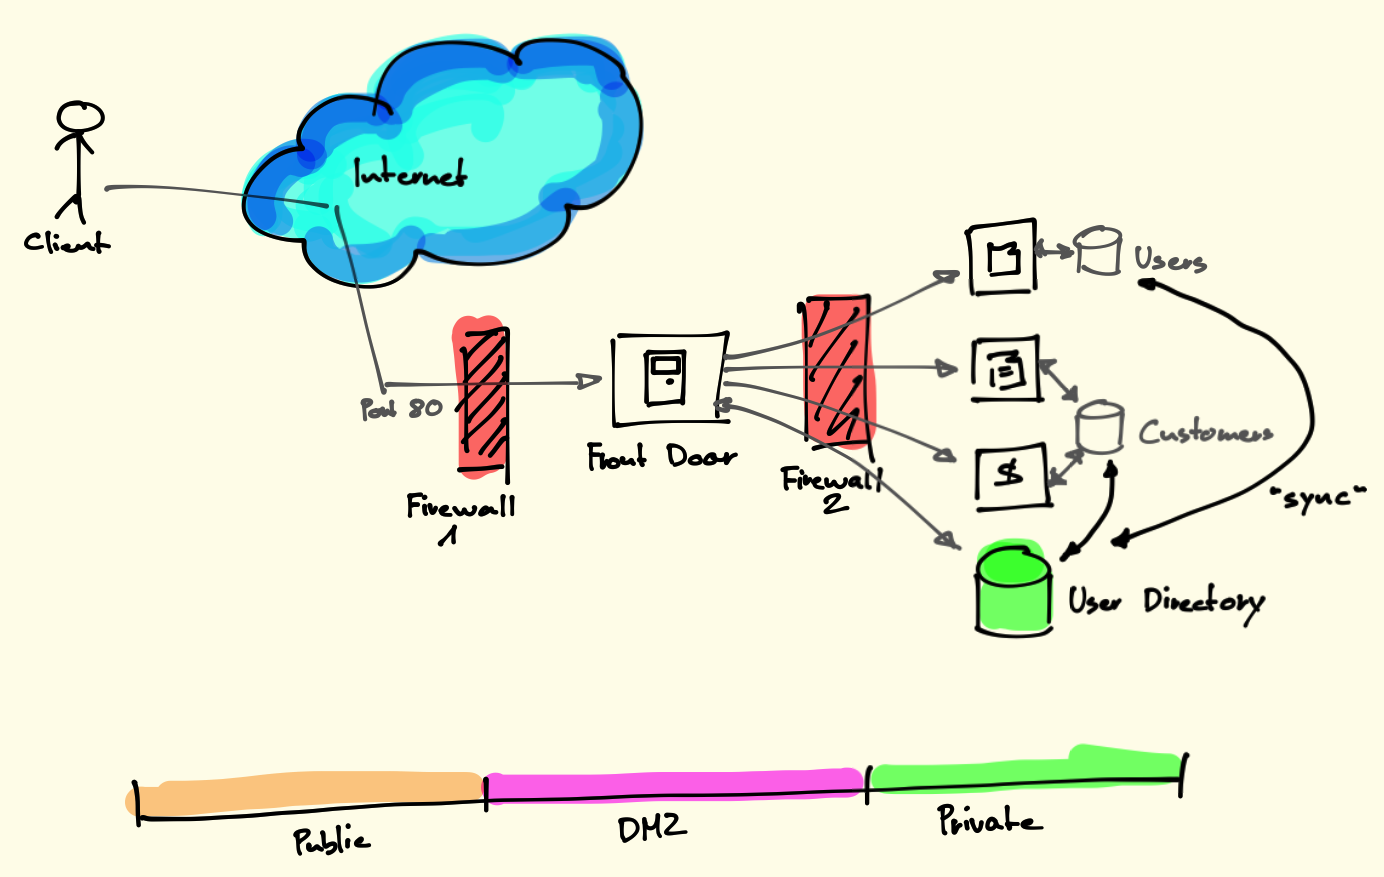
\includegraphics[width=12cm]{content/security/secure-internet-applications/images/front-door.png}
	\caption{Strutkureller Aufbau Front Door}
\end{figure}

Ein zentrales \emph{User Directory} ermöglicht das Authentifizieren von Benutzern.

\subsubsection*{Umsetzung}
\begin{enumerate}
	\item Es muss eine klare Repräsentation alle Benutzerinformationen gefunden werden. Dies gestaltet sich dann schwierig, wenn bestehende Komponenten mit bestehenden Benutzerdatenbanken integriert werden müssen.
	\item Die Autentication-Mechanismen müssen definiert werden (Username/Password, Username/Token usw. Siehe auch \ref{sec:ianda-requriements} ``\nameref{sec:ianda-requriements}'')
	\item Zugriffsberechtigungen müssen definiert werden. Auf Ebene der \emph{Front Door} kann bspw. allen Mitarbeitern Zugang gewährt werden. Später bei einzelnen Komponenten nur noch Ausgewählten (Siehe u. A. auch \ref{sec:accesscontrolmodels} ``\nameref{sec:accesscontrolmodels}'')
	\item Definition, wie Sessions im System weitergegeben werden sollen (Cookies? Header-Fields? Interne und externe Repräsentation? Siehe auch \ref{sec:security-session} ``\nameref{sec:security-session}'')
	\item Umsetzung des effektiven Session Contexts für die \emph{Front Door}
	\item Umsetzung eines \emph{Cookie Jars} für Cookies der internen Web- und Applikationsservern (Auch hier müssen entsprechende Sessions aufrechterhalten werden können)
	\item Gestaltung und Umsetzung der Anmelde- und Portalseite der \emph{Front Door}. Nicht vergessen: Single Sign Off. (Siehe auch \ref{sec:checkpoint} ``\nameref{sec:checkpoint}'')
\end{enumerate}

\subsection*{Vorteile}
\begin{itemize}
	\item Single Sign On und Off ermöglichen einfaches Sessionhandling über mehrere Systemkomponenten hinweg
	\item Ein Benutzerprofil über mehrere Systemkomponenten hinweg
	\item Einzelne Komponenten müssen sich nicht mehr um I\&A kümmern (analog \ref{sec:checkpoint} ``\nameref{sec:checkpoint}'')
	\item Wie beim \nameref{sec:integration-reverse-proxy} ein zentralisiertes Logging
\end{itemize}

\subsection*{Nachteile}
\begin{itemize}
	\item Sessiontimeouts zwischen \emph{Front Door} und effektiven Systemkomponenten
	\item Ein zentrales Verwalten der Benutzerdatenbank ist unumgänglich
	\item Synchronisation von Benutzerdatenbanken verschiedener Systemkomponenten kann aufwändig und fehleranfällig werden
\end{itemize}